\chapter{Position Control of the Base}
\label{cha:position_base}

Our main objective regarding the control of the base is to achieve a set point tracking as fast as physically possible, while maintaining a phase margin $\phi_m\approx$ 60° to ensure robustness.

\section{Controller Design}

To do so we designed a controller based on the Bode diagram of the model of the system in open loop, represented in the image below:

\image{./images/Chapter 3/Bode OL uncontrolled.png}

By looking at the pole-zero map below we can see that the dominant poles are the complex conjugate ones, which must be cancelled in order to speed up the response of the system.

\image{./images/Chapter 3/pzmap uncontrolled.png}

Even though the model itself presents a pole in the origin, an integral action in the controller is still needed in order to grant a zero steady state error, but doing so we drastically reduce the phase and make the system unstable.
To fix this issue we added two poles right before the anti resonance in order to get the desired phase margin and, for feasibility reasons, two poles right after the resonance which also have the function to lower the peak at $\approx 30 \frac{rad}{s}$.

Finally the overall gain of the controller is tweaked such that the crossing frequency is right before the anti-resonance, to get as much bandwidth as possible.

The controller transfer function is thus:

\begin{equation}
    C = 150 \frac{(s+7.43-24.5i)(s+7.43+24.5i)(s+3)^2}{s(s+22)^2(s+150)}
\end{equation}

And the Bode diagram of the controlled system in open loop and its pole-zero map are respectively:

\begin{figure}[H]
     \centering
     \begin{subfigure}{0.47\textwidth}
         \centering
         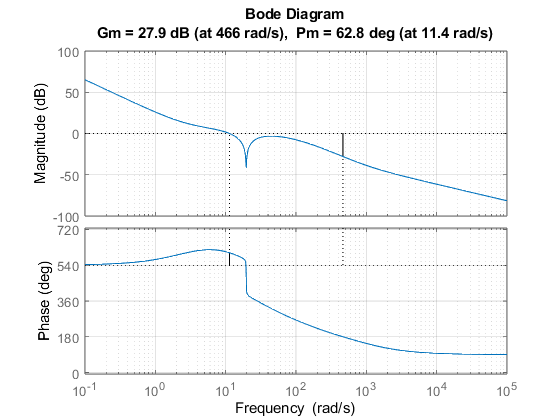
\includegraphics[width=\textwidth]{./images/Chapter 3/Bode OL controlled.png}
     \end{subfigure}
     \hfill
     \begin{subfigure}{0.47\textwidth}
         \centering
         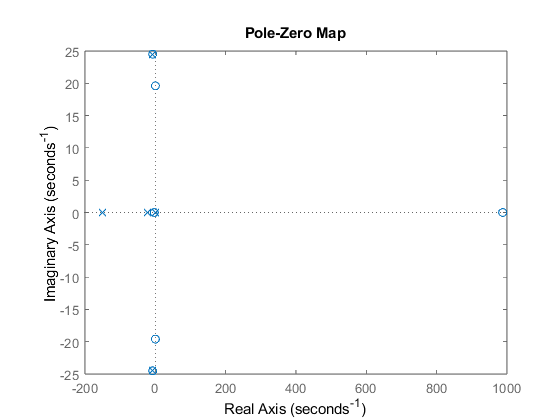
\includegraphics[width=\textwidth]{./images/Chapter 3/pzmap controlled.png}
     \end{subfigure}
\end{figure}


The overall control scheme is then:

\image{./images/Chapter 3/Control scheme.png}

\section{Validation}

Now that we have developed a control scheme, we have to verify that the closed loop system behaves accordingly to the specification imposed. 

\subsection{Step response}

\image{./images/Chapter 3/FBstepFire.png}      



\subsection{Frequency validation}

By testing the system with sinusoidal references at fixed amplitudes and different frequencies we were able to reconstruct a Bode diagram for the actual closed loop system. The comparison between the experimental one and the theoretical one can be seen in the plot below:

\image{./images/Chapter 3/Base FB fire controller Closed Loop.png}      

As we can see, at low frequencies the system is able to track the reference with small amplitude reduction up until $\approx 10 \, \frac{rad}{s}$ right before the anti-resonance, as expected.